\documentclass[11pt]{article}

\usepackage[margin=1in]{geometry}
\usepackage{amsmath,amssymb}
\usepackage{booktabs}
\usepackage{graphicx}
\usepackage{xcolor}
\usepackage{hyperref}
\usepackage{enumitem}
\usepackage{caption}
\usepackage{array}
\usepackage{float}
\usepackage{xurl}

\hypersetup{colorlinks=true, linkcolor=blue!50!black, urlcolor=blue!50!black}
\setlist{itemsep=2pt, topsep=4pt}
\usepackage{microtype}
\setlength{\emergencystretch}{3em}
\newcommand{\codeus}{\textunderscore\allowbreak}
\newcommand{\code}[1]{{\ttfamily\let\_\codeus #1}}

\title{Pollution Sources Upstream of the Stations,\\
       and Where the Benchmark Does Worst}
\author{Andrew Chincea \\ TDA Lab}
\date{November 2026}

\begin{document}
\maketitle

\begin{abstract}
Can we identify facilities that may pollute the rivers, such as factories, mines, wastewater plants
or data centres, and do they explain why the models do worse at some stations than at others? The
first part is possible with public data. After construction and other temporary permits are
removed, EPA's ECHO database lists $2{,}677$ permitted dischargers in the Upper and Lower Colorado
basins, and OpenStreetMap shows $122$ data-centre campuses in and
around the basin. Following each one downstream along the river network shows that $1{,}919$
dischargers and $19$ data-centre campuses drain past at least one of our water-quality stations.
EPA's StreamCat adds watershed measures of urban land, agriculture, mining, toxic-release and
Superfund sites. The second part is mostly no. Across stations, none of 33 such measures is
consistently related to where the graph model's error is: $20$ of $165$ measure-and-target pairs
reach $p<0.05$, against about $8$ expected by chance, and the only two that survive a
false-discovery correction point the other way (more hay and fertilizer upstream, less
specific-conductance error), which reflects geography rather than pollution. The error is instead
concentrated at a few stations whose problems have specific, mostly non-industrial causes the
model is not told about: releases from large dams (Lees Ferry, Verde below Bartlett Dam,
Greendale), a natural salt brine (the Dolores, $60\%$ of the specific-conductance error), a summer
reach depleted by irrigation diversions (DO), and two six-day records of a storm pulse on the San
Juan ($63\%$ of the turbidity error). In a few places a large discharge sits just upstream (the
Farmington wastewater plant $3$\,km above its station; the Glenwood Springs plant and hot springs
$6$--$9$\,km above theirs). Data centres are upstream of only four stations, at least $329$\,km
away, and the model already does relatively well at those stations.
\end{abstract}

% =====================================================================
\section{Question and short answer}

The benchmark predicts water temperature, dissolved oxygen (DO), specific conductance, pH and
turbidity at a station from season, a few terrain attributes, co-measured chemistry and the graph
of the river network, leaving each station out in turn. It does not know about anything that
enters the river between stations. This report asks two questions:
\begin{enumerate}
  \item Which possible pollution sources lie upstream of each station?
        (Sections~\ref{sec:data}--\ref{sec:sources})
  \item Do the stations where the model does worst have more of them?
        (Sections~\ref{sec:where}--\ref{sec:datacentres})
\end{enumerate}
Short answer: the sources can be identified and are listed per station in
\code{data/pollution/}, but they do not explain the error pattern. What explains it is a handful of
hydrologically unusual stations (Section~\ref{sec:why}).

% =====================================================================
\section{Data and method}\label{sec:data}

\paragraph{Permitted dischargers (EPA ECHO).} Every active Clean Water Act permit in the Upper and
Lower Colorado regions (2-digit HUC 14 and 15): $15{,}734$ records, with location, industry (SIC)
codes, major/minor status, permit components, design flow and toxic releases to surface water.
Records labelled construction stormwater ($5{,}700$, temporary building sites) are left out.
Records are counted once per facility (same name, location and category). Each remaining facility
is put in one category: municipal wastewater (POTW or sewerage), power plant, coal mine, metal or
uranium mine, other mining (sand, gravel, potash), oil and gas, manufacturing (factories), fish
hatchery, drinking-water plant, industrial stormwater or other individual permit. General-permit
coverages with no industrial code ($6{,}412$, mostly construction sites, dewatering and pipeline
tests that ECHO does not label as construction) are kept apart and left out of the totals.

\paragraph{Data centres (OpenStreetMap).} Buildings tagged as data centres in a box around the basin
($165$ features), grouped into $122$ campuses (same operator, within about 1\,km). OpenStreetMap is
crowd-sourced, so the list is incomplete, and a few small offices are mis-tagged.

\paragraph{Watershed measures (EPA StreamCat).} For each station's NHDPlus reach (found with the
USGS NLDI), StreamCat values for the whole upstream watershed: densities of permitted sites,
wastewater plants, Toxic Release Inventory and Superfund sites, mines and coal mines, dams and
canals; population, roads and septic systems; impervious, urban, crop, hay and barren land;
fertilizer and manure; irrigation; area burned 2014--2018; and the water-chemistry part of EPA's
Index of Watershed Integrity.

\paragraph{Wastewater share of flow.} The design flow of all municipal plants upstream, divided by
the station's mean discharge (22 of the 26 station nodes have discharge). The median is $2.5\%$.
Design flows overstate actual discharges, and reservoirs and diversions make this an indicator
rather than a mixing calculation.

\paragraph{Linking sources to stations.} Each facility is followed downstream from its location
along the MERIT Hydro flow directions (the grid the river graph is built on) until it reaches the
graph, then along the graph. Every station passed is \emph{downstream} of the facility, at the river
distance travelled. A facility is \emph{local} to the first station below it, i.e.\ it lies between
that station and the stations above. Facilities whose path never reaches a station drain into
another basin, a closed depression, or a river joining below the lowest station. Phoenix and
Tucson, for example, drain to the Gila, which joins the Colorado below Imperial Dam.

\paragraph{Where the error is.} The main benchmark's leave-one-station-out predictions (graph model:
$R^2$ $0.863$, $0.700$, $0.385$, $0.117$ and $0.104$ for the five targets). For each station:
its \emph{share} of the model's total squared error (equal station weights, so the shares add up
to $100\%$ and set $R^2$), its \emph{bias} (mean prediction minus observation), and how much of
its error is a constant offset.

\paragraph{Statistics.} Spearman rank correlation between each measure and the stations' error
shares, per target, with permutation $p$-values, a Benjamini--Hochberg false-discovery rate (FDR)
over the 33 measures of each target, and a partial correlation that removes drainage area. With
17--24 stations only correlations above about $0.45$--$0.5$ in size differ from zero at $p=0.05$,
and about one test in twenty passes by chance.

% =====================================================================
\section{What is upstream}\label{sec:sources}

\begin{table}[H]
\centering
\small
\caption{Possible pollution sources in the Colorado basin (HUC 14 and 15), and how many drain past
at least one water-quality station.}
\label{tab:sources}
\begin{tabular}{l rrr}
\toprule
Category & In the basin & Upstream of a station & Major permits upstream \\
\midrule
Municipal wastewater plants       & 363 & 271 & 57 \\
Power plants                      &  27 &  22 &  1 \\
Coal mines                        &  76 &  76 &  5 \\
Metal and uranium mines           &  57 &  30 &  3 \\
Other mining (sand, gravel, \ldots) & 316 & 267 &  0 \\
Oil and gas                       &  65 &  63 &  0 \\
Manufacturing (factories)         & 516 & 322 &  1 \\
Fish hatcheries                   &  17 &  13 &  0 \\
Drinking-water plants             &  85 &  77 &  0 \\
Industrial stormwater             & 890 & 541 &  1 \\
Other individual permits          & 265 & 237 &  4 \\
\midrule
All permitted dischargers         & $2{,}677$ & $1{,}919$ & 72 \\
Data-centre campuses (OSM)        & 122 &  19 &  -- \\
\bottomrule
\end{tabular}
\end{table}

The Upper Colorado basin is mostly upstream of some station; most of the Lower basin is not
(Figure~\ref{fig:map}). Coal mines (Price River, North Fork, Yampa and San Juan fields), oil and gas
(Uinta, Piceance and San Juan basins) and the large Las Vegas wastewater plants (about
$350$\,MGD of design flow, draining through Lake Mead) are all upstream of stations. The big
Lower-basin cities, Phoenix and Tucson, with many of the Lower basin's factories and most of its
data centres, drain elsewhere. The station above
Imperial Dam has the most upstream: $1{,}886$ dischargers and $560$\,MGD of municipal design flow,
two thirds of it from Las Vegas and St.~George.

\begin{figure}[tbp]
\centering
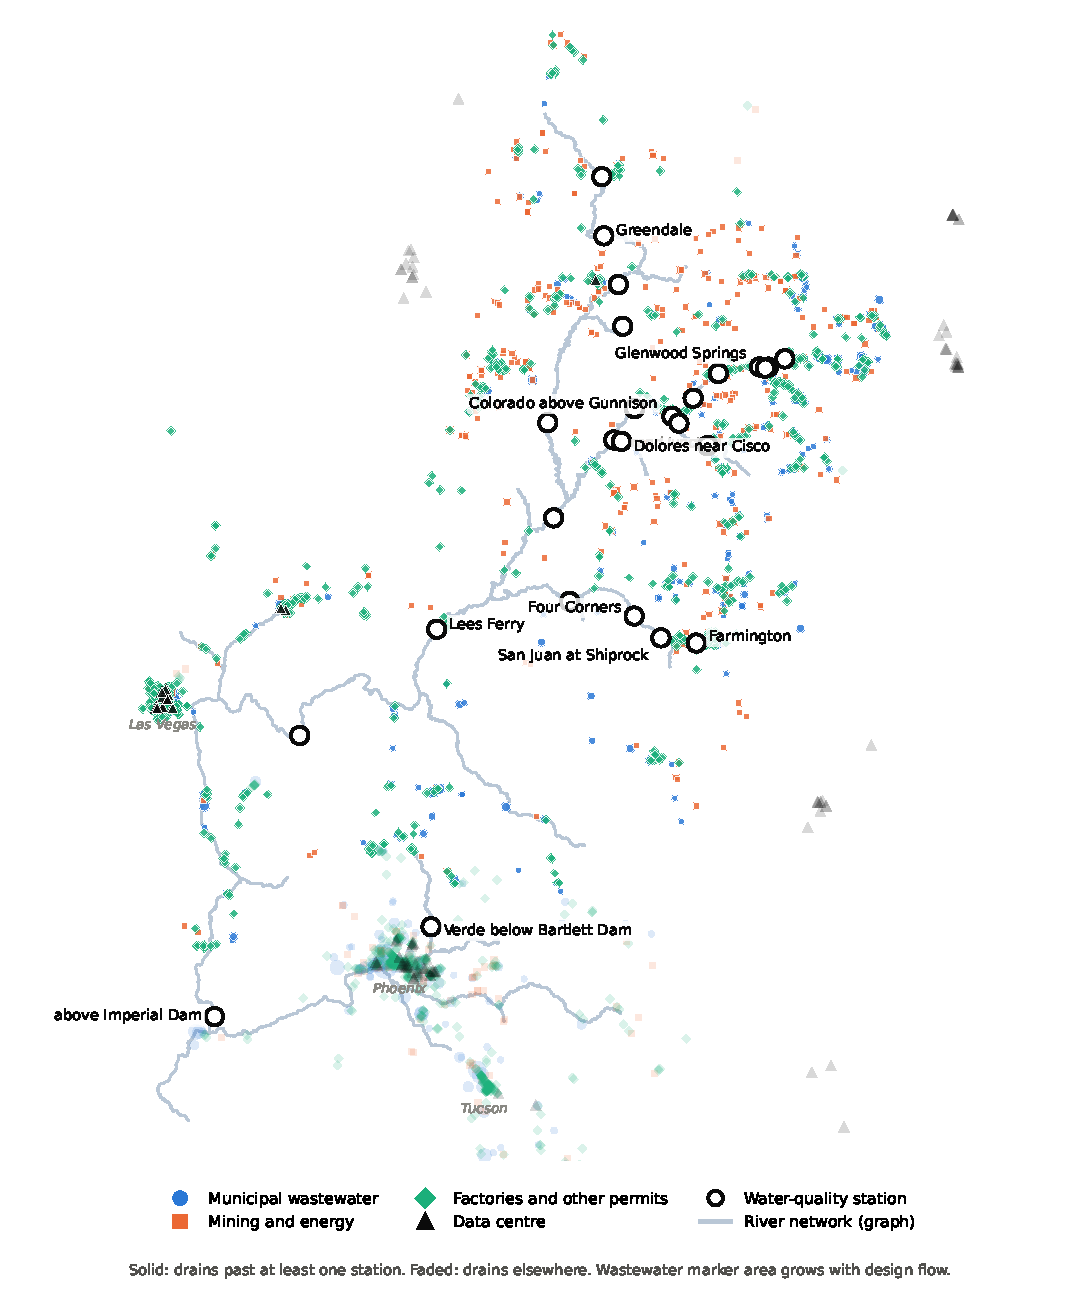
\includegraphics[width=0.92\textwidth]{figures/pollution_map.pdf}
\caption{Traced possible pollution sources and the water-quality stations. Solid markers drain past
at least one station; faded ones drain elsewhere. General-permit coverages without an industrial
code are not shown.}
\label{fig:map}
\end{figure}

% =====================================================================
\section{Where the error is, and what is upstream of those stations}\label{sec:where}

For every target, a few stations carry most of the graph model's error
(Figure~\ref{fig:error}): two stations give $31\%$ of the water-temperature error, three give $61\%$
of DO, one gives $60\%$ of specific conductance, and two give $63\%$ of turbidity.
Table~\ref{tab:cases} lists them with what lies upstream.

\begin{figure}[tbp]
\centering
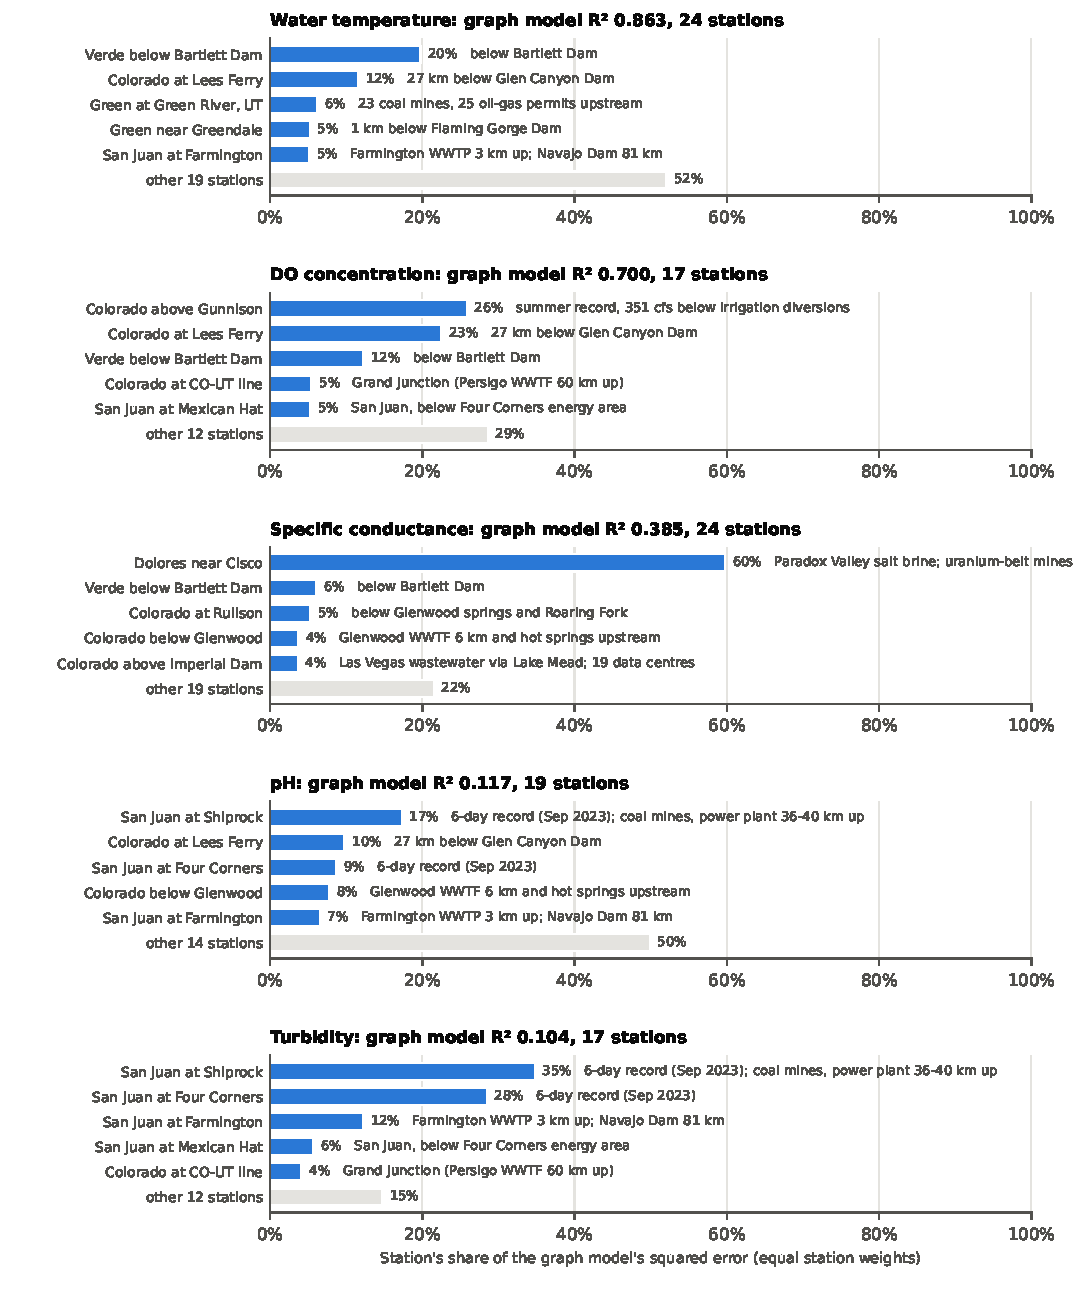
\includegraphics[width=\textwidth]{figures/pollution_error.pdf}
\caption{Each station's share of the graph model's squared error (the five largest per target),
with what lies upstream of it or is unusual about its record.}
\label{fig:error}
\end{figure}

\begin{table}[tbp]
\centering
\footnotesize
\caption{The stations that carry most of each target's error. Share: of the graph model's squared
error. Bias: mean prediction minus observation. Sources: traced permits, with river distance
upstream.}
\label{tab:cases}
\begin{tabular}{>{\raggedright\arraybackslash}p{2.6cm} >{\raggedright\arraybackslash}p{2.0cm}
                >{\raggedright\arraybackslash}p{4.6cm} >{\raggedright\arraybackslash}p{5.2cm}}
\toprule
Station & Share, bias & What is unusual & Permitted sources upstream \\
\midrule
Verde River below Bartlett Dam &
WT $20\%$, $+0.4$\,\textdegree C; DO $12\%$, $-1.2$\,mg/L; SC $6\%$ &
4\,km below Bartlett Dam: the annual temperature cycle is damped and shifted, so the error is in its
shape, not a constant offset &
33, all local: Payson ($2.8$\,MGD, 148\,km) and Cottonwood ($1.5$\,MGD, 198\,km) wastewater,
Page Springs fish hatchery (204\,km) \\
\addlinespace
Colorado River at Lees Ferry &
WT $12\%$; DO $23\%$, $+1.5$\,mg/L; pH $10\%$, $+0.25$ &
27\,km below Glen Canyon Dam, which releases water from deep in Lake Powell; observed DO and pH are
lower than the model predicts &
25 local, of which the dam's power plant (28\,km) and gravel and concrete plants at Page (44\,km);
$1{,}128$ upstream in all \\
\addlinespace
Green River near Greendale &
WT $5\%$, $-2.5$\,\textdegree C &
1\,km below Flaming Gorge Dam; the model is too cold by $2.5$\,\textdegree C on average &
36 local; nearest large plants 148--171\,km (Green River and Rock Springs, WY) \\
\addlinespace
San Juan River at Farmington &
WT $5\%$, $+1.9$\,\textdegree C; pH $7\%$; turbidity $12\%$ &
81\,km below Navajo Dam (cold releases); the Animas joins here &
119, all local: Farmington wastewater plant ($5.8$\,MGD) only 3\,km upstream; Aztec and Bloomfield
plants (30--35\,km); oil-field service firms \\
\addlinespace
Colorado River above the Gunnison at Grand Junction &
DO $26\%$, $-0.1$\,mg/L &
Summer-only record (1{,}885 hours, mean $22.9$\,\textdegree C) on a reach depleted by Grand Valley
irrigation diversions (mean $351$\,cfs); the model gets the mean right but not the daily DO swing
(station $R^2=0.05$) &
34 local: gravel pits (4--14\,km), Clifton wastewater plant ($2.5$\,MGD, 14\,km), coal mines at
Palisade (29\,km), oil and gas fields near De~Beque (50--75\,km) \\
\addlinespace
Dolores River near Cisco &
SC $60\%$, $-1{,}000$\,\textmu S/cm &
Natural salt brine enters in Paradox Valley (Section~\ref{sec:why}); observed mean
$2{,}082$\,\textmu S/cm, the saltiest station by far &
30, all local: uranium-belt mines around Uravan and Naturita (96--138\,km), coal mines near Nucla
(121--128\,km), Telluride wastewater ($2.1$\,MGD, 220\,km) \\
\addlinespace
San Juan River at Shiprock &
turbidity $35\%$; pH $17\%$ &
Only 6--7 days of record (11--17 September 2023), during a runoff pulse: discharge up to
$1{,}945$\,cfs (median $594$), turbidity up to $3{,}950$\,FNU &
45 local: Four Corners Power Plant (36\,km), San Juan and Navajo coal mines (37--40\,km), Bluffview
power plant (61\,km) \\
\addlinespace
San Juan River at Four Corners &
turbidity $28\%$; pH $9\%$ &
The same six days and pulse: discharge up to $2{,}625$\,cfs, turbidity up to $3{,}920$\,FNU &
10 local (Shiprock wastewater, 56\,km); the Shiprock sources above at 84--122\,km \\
\addlinespace
Colorado River below Glenwood Springs (above South Canyon Creek) &
pH $8\%$, $+0.17$; SC $4\%$, $-217$\,\textmu S/cm &
Below the Glenwood Springs thermal springs, a known salt source; the model is too fresh here and
too salty above the springs &
Glenwood Springs wastewater ($2.3$\,MGD, 6\,km) and the hot-springs pool discharge (9\,km) \\
\bottomrule
\end{tabular}
\end{table}

What these stations have in common is not industry. Six of the nine are tailwaters of large dams
or carry natural salt; two are six-day records of one storm pulse; one is a summer reach depleted
by diversions. Permitted sources are present upstream of all of them, as they are upstream of
almost every station, but in most cases they are small or far away compared with the obvious
cause. The exceptions where a discharge is large and close are Farmington and Glenwood Springs, and
possibly the Grand Junction reach, where a small river carries effluent and irrigation return flow
in summer.

% =====================================================================
\section{Do pollution sources explain the error across stations?}\label{sec:stats}

Figure~\ref{fig:heatmap} correlates every measure with the stations' error shares. Of the $165$
measure-and-target pairs, $20$ reach $p<0.05$ and $4$ reach $p<0.01$, against about $8$ and $2$
expected by chance. Only two survive the false-discovery correction, both for specific
conductance, and both point the other way. Stations with more hay and pasture upstream
($\rho=-0.66$, FDR $0.03$), or more fertilizer ($\rho=-0.58$, FDR $0.05$), have \emph{smaller}
errors. Hay and fertilizer are highest above the Green River stations (Wyoming hay meadows), the
Gunnison and the San Juan at Farmington, whose conductance the model predicts well. The stations
with the largest errors (Dolores, Verde, Rulison, Glenwood Springs) have little of either. The
correlation reflects where a station is, not what pollutes it.

\begin{figure}[tbp]
\centering
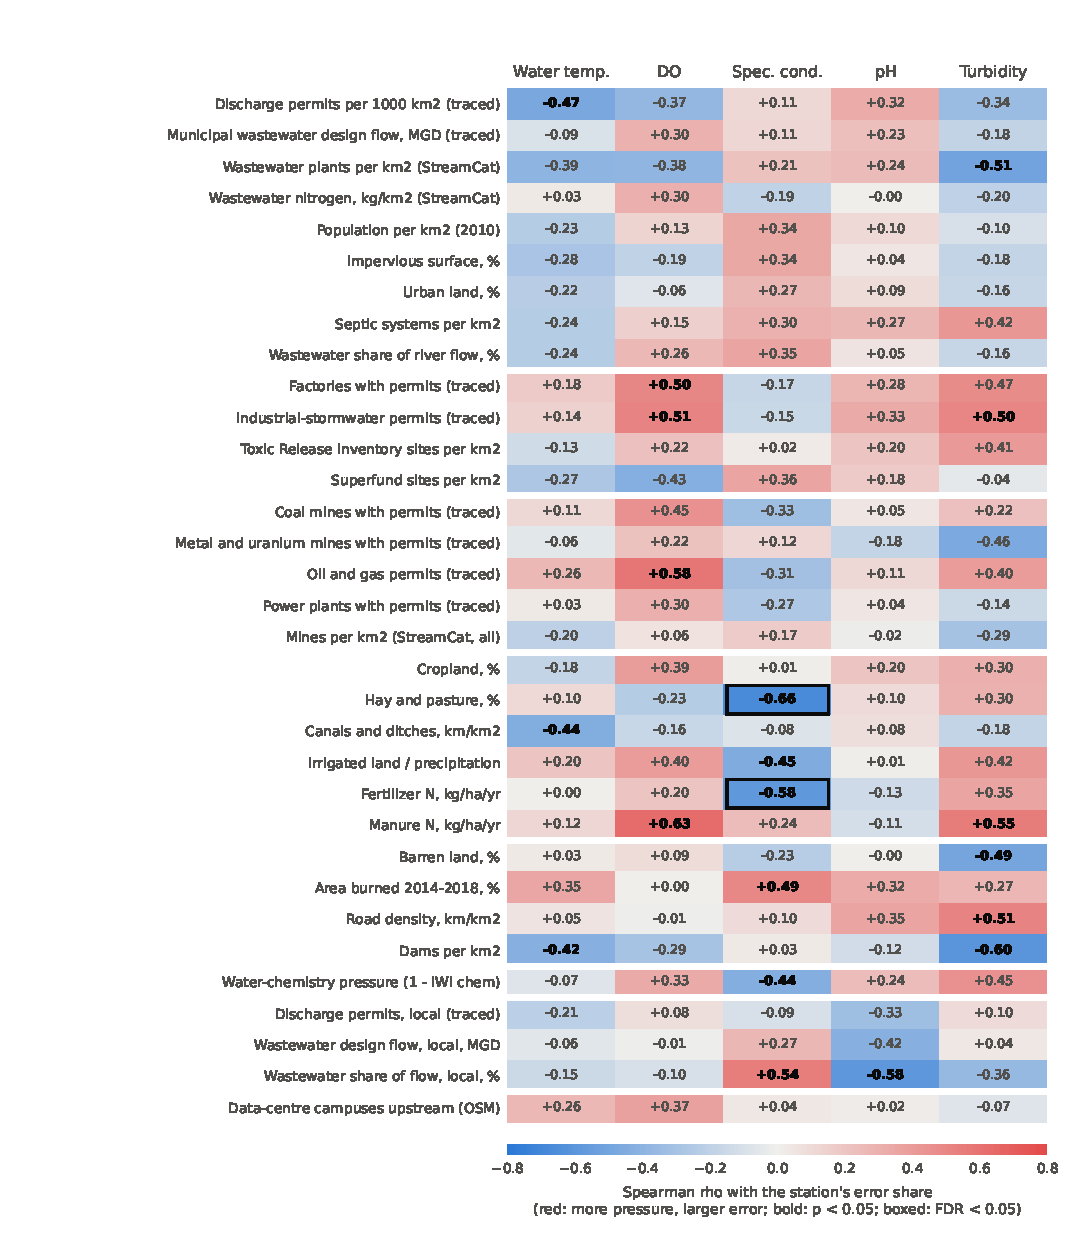
\includegraphics[width=0.86\textwidth]{figures/pollution_heatmap.pdf}
\caption{Spearman correlation between each measure upstream of a station and the station's share of
the graph model's error, per target (17--24 stations). Groups, top to bottom: wastewater and urban;
industry and toxics; mining and energy; agriculture and irrigation; land disturbance; overall
chemistry pressure; sources between the station and the next one up (local); data centres.}
\label{fig:heatmap}
\end{figure}

\begin{itemize}
  \item \textbf{Most other signals are geography or river size.} For DO, oil-and-gas permits
        ($\rho=0.58$), factories ($0.50$) and industrial stormwater ($0.51$) look related to the
        error, but these counts grow with drainage area. With area removed, they fall to $0.31$,
        $0.09$ and $0.16$. Manure ($0.63$, $0.53$ with area removed) is the one that holds. It
        is lowest at the clean headwater stations near Dotsero and Glenwood Springs and higher on the
        Gunnison, the lower main stem and the Verde, so it too separates headwaters from downstream
        rivers. For turbidity, more dams upstream go with
        less error ($\rho=-0.60$): dams trap sediment, so those stations are clear and easy to
        predict.
  \item \textbf{Wastewater share of flow.} The physically most direct measure shows no consistent
        relation. The full-upstream share has $|\rho|\le0.35$ for every target. The local share
        goes with larger specific-conductance error ($\rho=0.54$, $p=0.02$) but with smaller pH
        error ($\rho=-0.58$, $p=0.02$). Neither survives the correction, and they disagree in
        sign.
  \item \textbf{Local sources and the graph.} The graph model pulls each station towards its
        neighbours, so a source between a station and its neighbours should hurt the graph model
        more than Ridge, which ignores neighbours. The number of local permits and the local
        wastewater flow show no such pattern. The one lead is pH, where the graph model loses most
        to Ridge at stations with more Toxic Release Inventory sites ($\rho=0.65$, $p=0.004$),
        roads, people and impervious land ($\rho=0.48$--$0.56$) upstream. None of these survives
        the correction (smallest FDR $0.15$), so it is worth checking with more stations, not a
        result.
\end{itemize}

% =====================================================================
\section{Data centres}\label{sec:datacentres}

In and around the basin, data centres cluster in Phoenix, Las Vegas, Salt Lake City, Denver and
Albuquerque. Only Las Vegas drains to a monitored reach, together with two campuses in St.~George
and one in Vernal. Salt Lake City, Denver and Albuquerque are outside the basin, and Phoenix drains
to the Gila below our stations.

\begin{table}[H]
\centering
\small
\caption{Stations with data-centre campuses upstream, and their share of the graph model's error.}
\label{tab:dc}
\footnotesize\setlength{\tabcolsep}{4pt}
\begin{tabular}{l l r rrrrr}
\toprule
Station & Campuses & Nearest & \multicolumn{5}{c}{Share of the error} \\
        &          & (river km) & WT & DO & SC & pH & Turb. \\
\midrule
Colorado above Imperial Dam     & 19 (Las Vegas 17, St.~George 2) & 538 & $2\%$ & $4\%$ & $4\%$ & $2\%$ & -- \\
Green River at Green River, UT  & 1 (Vernal)                      & 329 & $6\%$ & $4\%$ & $1\%$ & $5\%$ & $3\%$ \\
Colorado at Gypsum Canyon       & 1 (Vernal)                      & 568 & $5\%$ & -- & $1\%$ & -- & -- \\
Colorado at Lees Ferry          & 1 (Vernal)                      & 889 & $12\%$ & $23\%$ & $1\%$ & $10\%$ & $<1\%$ \\
\bottomrule
\end{tabular}
\end{table}

The station with nearly all of the upstream data centres, above Imperial Dam, carries only
$2$--$4\%$ of each target's error. The one data-centre station with large shares, Lees Ferry, owes
them to Glen Canyon Dam; its only upstream data centre is almost 900\,km away. Data centres affect
water mainly through what they withdraw for cooling. What they discharge, typically cooling-tower
blowdown sent to the sewer, reaches the river as part of the wastewater plants' effluent, already
counted above. They do not explain the model's errors.

% =====================================================================
\section{Why the model does worst where it does}\label{sec:why}

The model knows the season, a few terrain attributes, the co-measured chemistry and its graph
neighbours. Where something between a station and its neighbours sets the water quality, the
station departs from what its neighbours imply, and the graph's smoothing pulls its prediction the
wrong way. In this basin the large inputs of that kind are mostly not permitted discharges:
\begin{itemize}
  \item \textbf{Dam releases.} Glen Canyon, Bartlett, Flaming Gorge and Navajo Dams release water
        drawn mostly from below the reservoir surface: cold in summer, mild in winter, sometimes
        low in oxygen. This drives the
        water-temperature, DO and pH errors at Lees Ferry, below Bartlett, at Greendale and partly
        at Farmington. The dam-tailwater terms tested in \code{r2\_experiments\_report.pdf} cut the
        water-temperature error at the two worst stations by three quarters (MSE $32.6\to7.4$ and
        $19.1\to4.3$).
  \item \textbf{Natural salt.} The Dolores picks up an estimated $205{,}000$ tons of salt a year in
        Paradox Valley, mostly from natural brine. Reclamation's Paradox Valley Unit pumps the brine
        and injects it deep underground. Injection stopped from March 2019 to June 2022 after an
        earthquake and has since run at a reduced rate, so the salt load has varied in recent
        years. Thermal springs at Glenwood Springs and Dotsero likewise deliver a large share of the
        upper Colorado's salt. No permit inventory captures these sources, and the Dolores alone is
        $60\%$ of the specific-conductance error.
  \item \textbf{Storm pulses in very short records.} The two San Juan stations each contribute one
        week, during which a runoff pulse raised turbidity to nearly $4{,}000$\,FNU. With equal
        station weights, those two weeks are $63\%$ of the turbidity error and $26\%$ of the pH
        error.
  \item \textbf{Water use.} Irrigation diversions leave the Colorado above the Gunnison at a
        few hundred cfs in summer, warm and with strong daily DO swings.
\end{itemize}
Counting facilities is a poor proxy for these. A count is not a load. Most permitted discharges
are small relative to river flow (median wastewater share $2.5\%$). With 17--24 stations, only
large effects can be seen.

% =====================================================================
\section{What could help}\label{sec:next}

\begin{itemize}
  \item \textbf{Process information rather than counts.} The features that did help target these
        mechanisms directly: dam-tailwater terms for water temperature ($+0.048$), and a runoff
        signal for turbidity ($+0.31$ for gradient boosting, $+0.21$ without the two San Juan
        records). Static counts of facilities are
        unlikely to help: three StreamCat measures offered for specific conductance in an earlier
        run gave $0.366$ against $0.385$ without.
  \item \textbf{Dam operations.} Release temperatures or depths from Reclamation for Glen Canyon,
        Flaming Gorge and Navajo Dams would let the model represent tailwaters directly.
  \item \textbf{Known salt sources.} A flag for the few reaches with known natural salt inflow
        (Paradox Valley, Glenwood and Dotsero springs) is physically justified, but it would rest
        on two or three stations.
  \item \textbf{Actual loads for the largest dischargers.} ECHO's discharge monitoring reports give
        monthly flows and concentrations. For the dozen largest plants near stations (Farmington,
        Glenwood Springs, Clifton, the Las Vegas plants), effluent loads relative to river flow
        would test the local-discharge explanation properly.
  \item \textbf{Record length.} Report turbidity and pH $R^2$ with and without the two six-day San
        Juan records, or weight stations by record length as a sensitivity check.
\end{itemize}

% =====================================================================
\section{Limitations}

Facility coordinates are addresses or centroids, not outfalls. Flow tracing on a 90\,m grid can
misroute a facility next to a confluence. Permits are not loads, and design flows overstate actual
flows. OpenStreetMap misses some data centres and mis-tags a few offices. StreamCat values are
rounded to four decimals and date from 2010 (population) to 2019 (land cover), with fires only to
2018. One graph node merges the Roaring Fork with the Colorado above it. Stations cover different
periods. All correlations are across 17--24 stations and are exploratory.

\paragraph{Data sources.} EPA ECHO Clean Water Act facility search
(\url{https://echo.epa.gov}); EPA StreamCat (\url{https://www.epa.gov/national-aquatic-resource-surveys/streamcat-dataset});
OpenStreetMap contributors, via the Overpass API (ODbL); USGS NLDI and NWIS; MERIT Hydro flow
directions. Bureau of Reclamation, Paradox Valley Unit
(\url{https://www.usbr.gov/projects/index.php?id=390}); USGS Scientific Investigations Report
2023--5094 on brine discharge to the Dolores River (\url{https://pubs.usgs.gov/publication/sir20235094});
Colorado Geological Survey, Information Series 49, on the Glenwood Springs and Dotsero thermal
springs.

\paragraph{Reproducibility.} \code{fetch\_pollution\_sources.py} downloads the public data to
\code{data/pollution/}. \code{build\_pollution\_sources.py} traces every source downstream
(\code{sources\_traced.csv}, \code{source\_links.csv}, \code{station\_sources.csv}).
\code{analyze\_pollution\_vs\_error.py} joins them with the main benchmark's errors
(\code{results/pollution/}). \code{make\_pollution\_figures.py} draws the figures.

\end{document}
